%----------------------------------------------------------------------------------------
%	PACKAGES AND OTHER DOCUMENT CONFIGURATIONS
%----------------------------------------------------------------------------------------

\documentclass{article}

\usepackage{fancyhdr} % Required for custom headers
\usepackage{lastpage} % Required to determine the last page for the footer
\usepackage{extramarks} % Required for headers and footers
\usepackage[usenames,dvipsnames]{color} % Required for custom colors
\usepackage{graphicx} % Required to insert images
\usepackage{subcaption} % Another library for images
\usepackage{listings} % Required for insertion of code
\usepackage{courier} % Required for the courier font
\usepackage{amsmath}
\usepackage[color,matrix,arrow]{xy}

% Margins
\topmargin=-0.45in
\evensidemargin=0in
\oddsidemargin=0in
\textwidth=6.5in
\textheight=9.0in
\headsep=0.25in

\linespread{1.1} % Line spacing

% Set up the header and footer
\pagestyle{fancy}
\rhead{\firstxmark} % Top right header
\lfoot{\lastxmark} % Bottom left footer
\cfoot{} % Bottom center footer
\rfoot{Page\ \thepage\ of\ \protect\pageref{LastPage}} % Bottom right footer
\renewcommand\headrulewidth{0.4pt} % Size of the header rule
\renewcommand\footrulewidth{0.4pt} % Size of the footer rule

\setlength\parindent{0pt} % Removes all indentation from paragraphs

%----------------------------------------------------------------------------------------
%	CODE INCLUSION CONFIGURATION
%----------------------------------------------------------------------------------------

\definecolor{Lava}{rgb}{0.81,0.06,0.13} 
\definecolor{Green}{rgb}{0.11,0.35,0.02}
\definecolor{Purple}{rgb}{0.59,0.44,0.84}
\lstloadlanguages{Python} % Load Perl syntax for listings, for a list of other languages supported see: ftp://ftp.tex.ac.uk/tex-archive/macros/latex/contrib/listings/listings.pdf
\lstset{language=Python, 
        frame=single, % Single frame around code
        basicstyle=\bf\ttfamily, % Use small true type font
        keywordstyle=[1]\color{Blue}\bf, % Perl functions bold and blue
        keywordstyle=[2]\color{Purple}\bf, % Perl function arguments purple
        keywordstyle=[3]\color{Blue}\underbar, % Custom functions underlined and blue
        identifierstyle=, % Nothing special about identifiers                                         
        commentstyle=\usefont{T1}{pcr}{m}{sl}\color{Green}\small, % Comments small dark green courier font
        stringstyle=\color{Lava}, % Strings are purple
        showstringspaces=false, % Don't put marks in string spaces
        tabsize=5, % 5 spaces per tab
        %
        % Put standard Perl functions not included in the default language here
        morekeywords={rand},
        %
        % Put Perl function parameters here
        morekeywords=[2]{on, off, interp},
        %
        % Put user defined functions here
        morekeywords=[3]{test},
       	%
        morecomment=[l][\color{Blue}]{...}, % Line continuation (...) like blue comment
        numbers=left, % Line numbers on left
        firstnumber=1, % Line numbers start with line 1
        numberstyle=\tiny\color{Blue}, % Line numbers are blue and small
        stepnumber=5 % Line numbers go in steps of 5
}

\newcommand\boldblue[1]{\textcolor{blue}{\textbf{\textit{#1}}}} % bold blue text


%----------------------------------------------------------------------------------------
%	TITLE PAGE
%----------------------------------------------------------------------------------------

\title{
\vspace{2in}
\textmd{\textbf{DMO Computing Project 2017}}\\
\vspace{0.1in}\large{\textit{Prof. Marc Noy}}
\vspace{3in}
}

\author{\textbf{Emily Daykin, Travis Dunlop, Laurits Marschall}}

%----------------------------------------------------------------------------------------

\begin{document}

\clearpage\maketitle
\thispagestyle{empty}

%----------------------------------------------------------------------------------------
%	TABLE OF CONTENTS
%----------------------------------------------------------------------------------------

%\setcounter{tocdepth}{1} % Uncomment this line if you don't want subsections listed in the ToC

\newpage
\setcounter{page}{1}

%\tableofcontents
%\newpage

%----------------------------------------------------------------------------------------
%	Description of Algorithm
%----------------------------------------------------------------------------------------

\section*{Tasks 1 \& 2}

\textbf{\underline{Goal}}: To measure the minimum distance between two strings, X and Y. The edit distance is defined by the weighted  cost of the operations necessary to transform X into Y. Three different operations are used to transform the string. A letter can be \textit{inserted} into X, \textit{deleted} from X, or \textit{substituted} by a different one. Respective costs (I, D, S) are assigned to all three operations. The aim is to design an algorithm that finds the minimum cost necessary to transform X into Y. 

\qquad To compute this, we took a \textbf{dynamic programming} approach.  First we calculate the minimum edit distance between the two final characters in the strings, then the last two characters, then last three etc. At each step we use the previously 'memoized' optimal solutions.  Finally, we are left with comparing the two complete strings with the minimum edit distance computed.

\qquad The algorithm solves the problem by constructing three matrices, all of equal size, with each letter of Y as columns headings and that of X as rows, with one added 'end' row and column. The first matrix (\textit{matches}) compares each letter of X and Y. If they match, the cell is 0 and 1 otherwise.  The second matrix (\textit{min cost}) stores the accumulated minimum cost to reach the end of the transformation process. The third matrix (\textit{best}) contains the next step in the optimal path, both in English (i.e. 'match A') and as the index of the next value of the matrix (i.e. (3, 4)).

\qquad The algorithm first computes the \textit{matches} matrix, then fills out \textit{min cost} and \textit{best} iteratively from the last to the first cell, utilizing the 'memoized' solutions.  Once computed, the minimum overall cost is the first cell in \textit{min cost} and the corresponding path is found by following the steps given in \textit{best}.
\\\\
For any given cell $(i, j) \, i \leq n, \, j \leq m $, we choose the option of minimum cost:
\begin{itemize}    
    	\item insert the letter of Y in front of the letter of X and move right in the matrix to the next letter in Y but not in X. (cost $= I + min \, cost[i, j+ 1]$) 
    	\item delete the letter of X and move down in the matrix to the next letter of X but not of Y. \\ (cost $= D + min\,cost[i+1, j]$)
	\item match (if possible) the two letters and move diagonally down and to the right within the matrix.	\\ (cost $= min\,cost[i+1, j+1]$)
    	\item substitute the letter of X by the letter of Y. Since the two letters match after this substitution, move diagonally down and to the right in the matrix.  (cost $= S + min\,cost[i+1, j+1]$)
\end{itemize}

Note that our algorithm includes the cost of each action as a parameter, so Task 1 is solved by choosing default values, and Task 2 is solved by setting the parameters to appropriate values.
\\\\
\textbf{\underline{Steps of the algorithm} (to be referenced in the code comments below):}

\begin{enumerate}
\item Initialize matrix \textit{matches} with value 0 if letters of X and Y match, 1 otherwise (the final cell is always set to 0)
	\begin{itemize}
	 \item[] \textit{matches} = \bordermatrix{~ & A & B & C & A & end \cr
                  		A & 0 & 1 & 1 & 0 & 1 \cr
                  		B & 1 & 0 & 1 & 1 & 1 \cr
                  		B & 1 & 0 & 1 & 1 & 1 \cr
                  		C & 1 & 1 & 0 & 1 & 1 \cr
                  		A & 0 & 1 & 1 & 0 & 1 \cr
                  		C & 1 & 1 & 0 & 1 & 1 \cr
                  		end & 1 & 1 & 1 & 1 & 0 \cr}
	\end{itemize}
	\item Initialize matrices \textit{min cost} and \textit{best}, with the same size and labels as \textit{matches}.
	\item Set the last row and column of \textit{min cost} and \textit{best} to initial values. If one string is empty, then the only option is to either delete or insert the other string.
	\item Iterate from the bottom right corner to the top left corner, at each step using the \textit{solve} function to compare the four options and choose the best.  This populates the other two matrices.
	\item We are left with the following \textit{min cost} and \textit{best} matrices.
	\begin{itemize}
	\item[] \textit{min cost} = \bordermatrix{~ & 	A & B & C & A & end \cr
                  					A & \boldblue{2} & 3 & 4 & 5 & 6 \cr
                  					B & 2 & 2 & 3 & 4 & 5 \cr
                  					B & 2 & 1 & 2 & 3 & 4 \cr
                  					C & 3 & 2 & 1 & 2 & 3 \cr
                  					A & 2 & 2 & 2 & 1 & 2 \cr
                  					C & 3 & 2 & 1 & 1 & 1 \cr
                  					end & 4 & 3 & 2 & 1 & 0 \cr}
	\end{itemize}
		 \textit{best} = \bordermatrix{~ & 	A & B & C & A & end \cr
                  					A & \boldblue{match\,A} & delete\,A & delete\,A & delete\,A & delete \,A \cr
                  					B & substitute \,B \,for\, A & \boldblue{delete \,B} & delete \,B & delete \,B & delete \,B \cr
                  					B & insert \,A & \boldblue{match\, B} & delete \,B & delete\, B & delete \,B \cr
                  					C & delete\, C & insert \,B & \boldblue{match \,C} & delete \,C & delete \,C \cr
                  					A & match \,A & substitute\, A \,for \,B & delete \,A & \boldblue{match \,A} & delete \,A \cr
                  					C & insert \,A & insert \,B & match \,C & substitute \,C \,for\, A & \boldblue{delete \,C} \cr
                  					end & insert \,A & insert \,B & insert \,C & insert \,A & \boldblue{insert end} \cr}

	Note, for visual clarity, we excluded the index of the next node in \textit{best} matrix.
	\item The minimum edit distance is the first value of \textit{min cost} (in this case 2, shown in blue above).  
	\item Return the corresponding set of instructions by following the path from the first value of \textit{best} until the end is reached.  In this case, \textit{match A} (move diagonal), \textit{delete B} (down), \textit{match B} (diagonal), \textit{match C} (diagonal), \textit{match A} (diagonal), \textit{delete C} (down), \textit{insert end} (shown in blue above). 

\end{enumerate}


\begin{lstlisting}
def edit_distance(x, y, D=1, I=1, S=1): 
# Define a function of strings X and Y and cost of each operation
    n = len(x)      # Define n as the length of string X
    m = len(y)      # Define m as the length of string Y
    rows = list(x) + ['end']                              
# Set each matrix row heading as X's characters, with added row 'end' 
    columns = list(y) + ['end']                        
# Set each matrix column heading as Y's characters, with added column 'end'
    
    matches = np.zeros((n+1,m+1), dtype = int) #Initialise the matrix "matches"
    min_cost = matches.copy()                             
# Create a duplicate "matches" matrix called "min_cost" (step 3 above)
    best = matches.copy().astype(np.object)               
# Create a duplicate "matches" matrix called "best"
    
    for i,a in enumerate(rows):                # For each row element
        for j,b in enumerate(columns):         # and each column element:
            if a != b:       # if the two strings' characters don't match:
                matches[i,j] = 1  
                # insert 1 in the cell (all others will remain zero)
    
    for i,a in enumerate(rows):     # For each row element
        min_cost[i, m] = (n - i) * D                      
#  fill "min_cost"'s last column with descending costs of D
        best[i,m] = ('delete ' + a, i+1, m)               
#  fill "best" with the tuple listing 'delete' row, and new cell indices 
    for j,b in enumerate(columns):   # For each column element 
        min_cost[n, j] = (m - j) * I                      
#  fill "min_cost"'s last row with descending costs of I
        best[n,j] = ('insert ' + b, n, j+1)               
#  fill "best" with the tuple listing 'insert' column, and new cell indices 
    
    def solve(i, j):        # Create a function of indices where
        a = rows[i]         # a is each of the rows, and
        b = columns[j]      # b each of the columns
        d_cost = D + min_cost[i+1,j]   # Set d_cost as given deletion cost 
        i_cost = I + min_cost[i,j+1]   # Set i_cost as given insertion cost 
        s_cost = S * matches[i,j] + min_cost[i+1,j+1]     
# Set s_cost as given substitution cost times 0 (match) or 1 (no match)
        
        c_min = min(d_cost, i_cost, s_cost)               
# Set c_min as the minimum cost of the above 3 operations
        min_cost[i,j] = c_min                             
# Set each value in "min_cost" as the least expensive operation (step 6 above)
        
        if d_cost == c_min:      # If deletion is cheapest
            best[i,j] = ('delete ' + a, i+1, j)           
# Fill tuple with command and the next cell to go to (downwards) in "best"
        elif i_cost == c_min:   # If insertion is cheapest
            best[i,j] = ('insert ' + b, i, j+1)           
# Fill tuple with command and the next cell to go to (rightwards) in "best"
        else:    # If substitution is cheapest
            if matches[i,j] == 0:     # and if the X and Y letter do match:
                best[i,j] = ('match ' + b, i+1, j+1)      
#   fill tuple with command and the next cell to go to (south-east) in "best"
            else:     # if X and Y letter do not match:
                best[i,j] = ('substitute ' + a + ' for ' + b, i+1, j+1) 
#   fill tuple with command and the next cell to go to (south-east) in "best"

    for i in range(n-1, -1, -1):                          
# For each row, move downwards decreasing value by 1 
        for j in range(m-1, -1, -1):                      
# For each column, move rightwards decreasing value by 1 
            solve(i,j)                                    
# Fill in "best" matrix as above (step 8 above)
            
    i, j = (0, 0)    # Initialise at i = j = 0
    solution = []     # Create an empty list called "solution"
    
    while i < n + 1 and j < m + 1:                        
# For each row and column within n and m limits,
        step = best[i,j]                                  
#   define "step" to give the corresponding tuple in the "best" matrix
        solution.append(step[0])   # add operation conducted to "solution"
        i = step[1]                # set i as the new current row
        j = step[2]                # set j as the new current column
    
    return(solution, min_cost[0,0])                       
# Give the optimum path and total minimum edit distance to transform X into Y!   
\end{lstlisting}

%----------------------------------------------------------------------------------------
%	PROBLEM 2
%----------------------------------------------------------------------------------------



%----------------------------------------------------------------------------------------
%	PROBLEM 3
%----------------------------------------------------------------------------------------

\section*{Task 3}

\begin{lstlisting}
x = 'ACTACTAGATTACTTACGGATCAGGTACTTTAGAGGCTTGCAACCA'
y = 'TACTAGCTTACTTACCCATCAGGTTTTAGAGATGGCAACCA'
\end{lstlisting}

\textbf{Unpenalized Version (D = I = S = 1):} \\
\textbf{Minimum Edit Distance:}  10 \\
\textbf{Path:}  delete A, delete C, match T, match A, match C, match T, match A, match G, substitute A for C, match T, match T, match A, match C, match T, match T, match A, match C, substitute G for C, substitute G for C, match A, match T, match C, match A, match G, match G, match T, delete A, delete C, match T, match T, match T, match A, match G, match A, delete G, match G, substitute C for A, match T, substitute T for G, match G, match C, match A, match A, match C, match C, match A, insert end \\

\textbf{Penalized Version (D = I = 2, S = 1):} \\
\textbf{Minimum Edit Distance:}  15 \\
\textbf{Path:}  delete A, delete C, match T, match A, match C, match T, match A, match G, substitute A for C, match T, match T, match A, match C, match T, match T, match A, match C, substitute G for C, substitute G for C, match A, match T, match C, match A, match G, match G, match T, delete A, delete C, match T, match T, match T, match A, match G, match A, delete G, match G, substitute C for A, match T, substitute T for G, match G, match C, match A, match A, match C, match C, match A, insert end \\

\begin{lstlisting}
x = 'AASRPRSGVPAQSDSDPCQNLAATPIPSRPPSSQSCQKCRADARQGRWGP'
y = 'SGAPGQRGEPGPQGHAGAPGPPGPPGSDG'
\end{lstlisting}

\textbf{Unpenalized Version (D = I = S = 1):} \\
\textbf{Minimum Edit Distance:}  37 \\
\textbf{Path:}  delete A, delete A, delete S, delete R, delete P, delete R, match S, match G, substitute V for A, match P, substitute A for G, match Q, delete S, substitute D for R, substitute S for G, substitute D for E, match P, insert G, substitute C for P, match Q, substitute N for G, substitute L for H, match A, insert G, match A, delete T, match P, substitute I for G, match P, substitute S for P, substitute R for G, match P, match P, delete S, delete S, substitute Q for G, match S, delete C, delete Q, delete K, delete C, delete R, delete A, match D, delete A, delete R, delete Q, delete G, delete R, delete W, match G, delete P, insert end \\

\textbf{Penalized Version (D = I = 2, S = 1):} \\
\textbf{Minimum Edit Distance:}  58 \\
\textbf{Path:}  delete A, delete A, delete S, delete R, delete P, delete R, match S, match G, substitute V for A, match P, substitute A for G, match Q, substitute S for R, substitute D for G, substitute S for E, substitute D for P, substitute P for G, substitute C for P, match Q, substitute N for G, substitute L for H, match A, substitute A for G, substitute T for A, match P, substitute I for G, match P, substitute S for P, substitute R for G, match P, match P, delete S, delete S, substitute Q for G, match S, delete C, delete Q, delete K, delete C, delete R, delete A, match D, delete A, delete R, delete Q, delete G, delete R, delete W, match G, delete P, insert end \\


%----------------------------------------------------------------------------------------
%	PROBLEM 4
%----------------------------------------------------------------------------------------

\section*{Task 4}
\begin{figure}[h!]
  \centering
  \begin{subfigure}[b]{0.45\linewidth}
    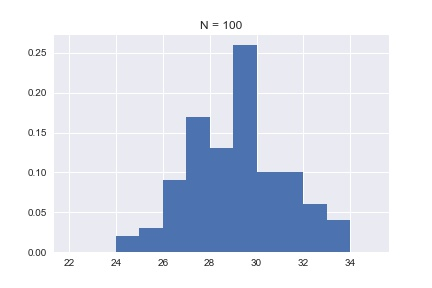
\includegraphics[width=\linewidth]{Edit_Distance_Histogram_100.jpg}
    \caption{mean: 28.7 - sample variance: 4.18}
  \end{subfigure}
  \begin{subfigure}[b]{0.45\linewidth}
    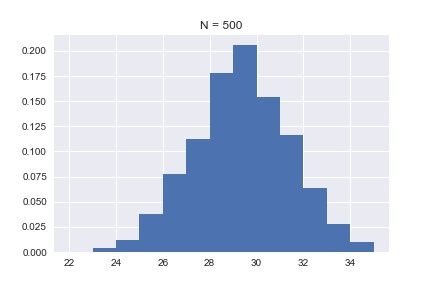
\includegraphics[width=\linewidth]{Edit_Distance_Histogram_500.jpg}
    \caption{mean: 28.8 - sample variance: 4.25}
  \end{subfigure}
  \begin{subfigure}[b]{0.45\linewidth}
    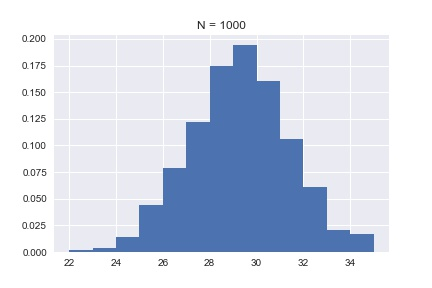
\includegraphics[width=\linewidth]{Edit_Distance_Histogram_1000.jpg}
    \caption{mean: 28.8 - sample variance: 4.68}
  \end{subfigure}
  
  \label{fig:coffee}
\end{figure}

Shown above are three histograms of minimum edit distance of N pairs of strings of length 50.  To generate the strings we choose equally randomly between \{A, B, C, D\}.  If we were interested in the case when the characters are not equally represented, we would simply change the weight in our selection for the letters.  For example, we generate a standard uniform pseudo-random variable and depending on which region its values lies in, we choose a letter.  The size of the decision regions is the probability we would choose that value.

\section*{Proof of Correctness}

We will build up the proof of correctness through induction.  First we consider the base case when we compare two empty strings, which has minimum edit distance zero.  Our algorithm creates the following 'best' matrix and concludes that the minimum cost is zero.
\begin{align*}
best = \bordermatrix{~ & end \cr
                  		end & insert\,end \cr}
\end{align*}

For the case when only one string is empty, by inspection we realize the minimum cost is to either delete or insert the entire string.  This case is represented in our algorithm by initializing the values of the last row and last column of our matrices. 
\begin{align*}
best = \bordermatrix{~ & & A & B & end \cr
                  		end & \hdots & insert \, A & insert\,B & insert\,end  \cr} \qquad
best = \bordermatrix{~ & end \cr
				 & \vdots \cr
				 A & delete \, A \cr
				 B & delete \, B \cr
                  		 end & insert\,end \cr}
\end{align*}

We now consider the simplest case when both X and Y are non-empty, when they each have one character. After initializing the last row and column, our algorithm computes all (reasonable) possibilities to transform the one character string into the other.  It compares 4 options: delete, insert, substitute or match (if possible).
\begin{align*}
best = \bordermatrix{~ & B & end \cr
				 B & * & delete \, B \cr
                  		 end & insert \, B & insert\,end  \cr}
\end{align*}

The value at the asterisk will be set as the minimum between the four options.  Note here, when we compute the total cost of the decision, we add the cost of the immediate decision plus the minimum cost of the next state.  In this way, we use the previously computed 'memoized' solutions under the dynamic programming framework.  Now, through induction, we can extend this decision framework directly to strings of arbitrary length.  
\begin{align*}
best = \bordermatrix{~ & B & A & \hdots \cr
				 A & * & delete \, B & \hdots \cr
                  		 C & insert \, B & substitute\,C\,for\,A  & \hdots \cr
		 		 \vdots & \vdots & \vdots & \ddots \cr}
\end{align*}

Above we see an example of a beginning of a comparison of two strings.  The decision at the asterisk is only determined by the minimum cost of the next immediate decision and the minimum cost of the corresponding next state.

\section*{Proof of Complexity}

In order to compute the minimum distance, we need to generate the three m by n matrices.  It takes constant time to fill out any individual value since we leverage previously memoized solutions. Therefore to fill out the matrices, it takes $O(mn)$ time. \\

Once the matrices are created, we also need to find the minimum path.  In the worst case, (delete all characters and then insert) this takes $O(m+n)$ time. \\

The $O(m+n)$ is swallowed by the more complex term, so in total the algorithm is run in $O(mn)$ time.



\end{document}